%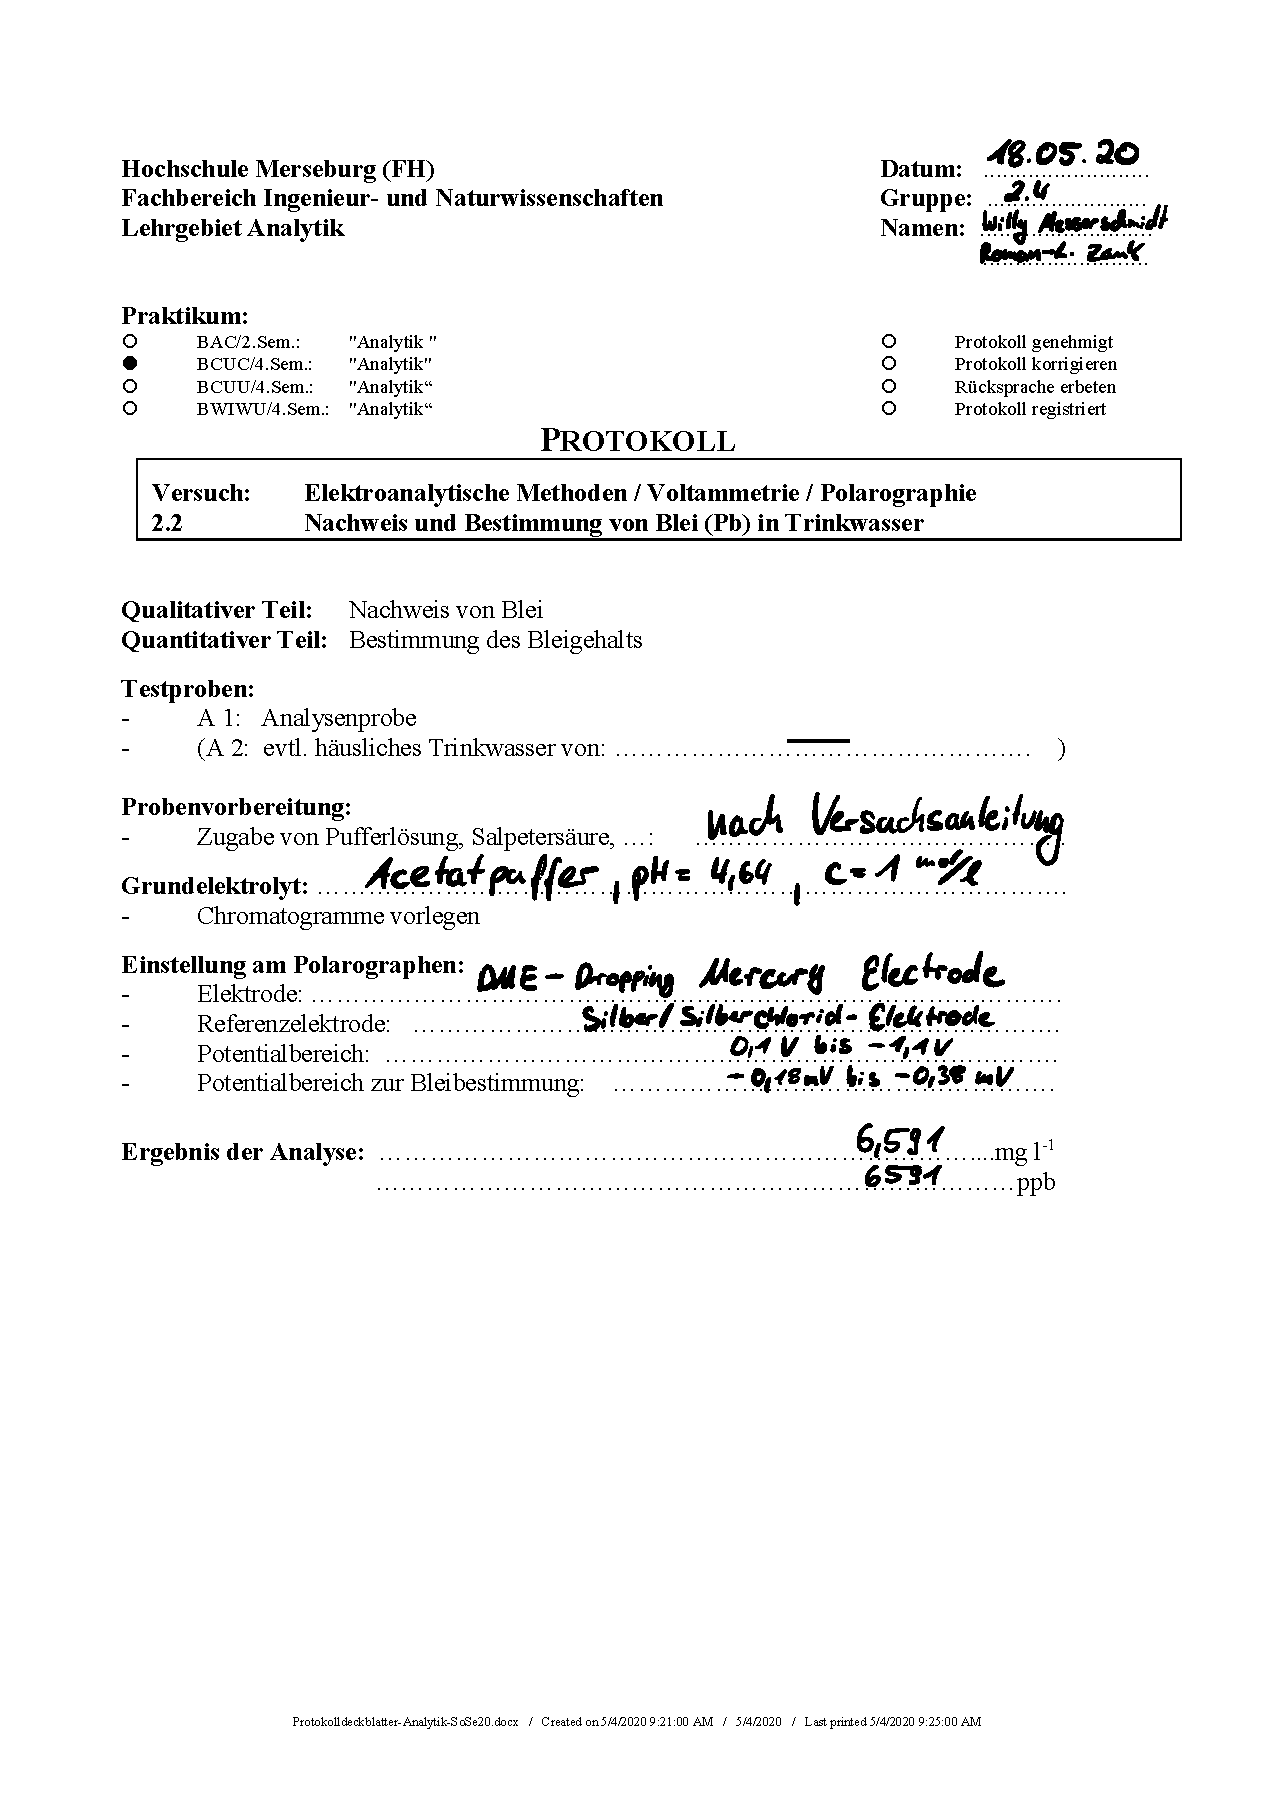
\includepdf[]{Deckblatt}
\pagebreak
\section{Einleitung}
\label{sec:einleitung}
Im folgenden Protokoll werden generierte Messdaten zum Versuch \textit{WÜP} ausgewertet. Ziel ist es mithilfe der erklärenden Videos zum Praktikum und Mittels der gegebenen Messdaten Aussagen über den Wärmeübergangsprozess zu treffen. Untersucht werden hierfür zwei Wärmetauscher, welche in Reihen- und Parallelschaltung vorliegen. Über Parameter wie der übertragenen Wärme, der \textsc{Reynolds}-, \textsc{Prandtl}- und \textsc{Nusselt}-Zahl, sowie des Wärmeübergangs- und des Wärmedurchgangskoeffizienten werden beide Schaltungen mit den entsprechenden Betriebsvorgaben miteinander verglichen. 





